%%%%%%%%%%%%%%%%%%%%%%%%%%%%%%%%%%%%%%%%%%%%%%%%%%%%%%%%%%%%%%%%%%%%%%%%
\chapter{Representation Analysis for NLP}
%%%%%%%%%%%%%%%%%%%%%%%%%%%%%%%%%%%%%%%%%%%%%%%%%%%%%%%%%%%%%%%%%%%%%%%%
With the advent of neural methods for NLP systems, it became significantly more difficult to explicitly and totally control the inner behavior of the model, which was straightforward in \textit{symbolic} methods, as well as in purely statistical ones, to a certain extent. 

Analyzing the weights and activations of the intermediate layers of neural NLP models is the purpose of the \textit{interpretability} field \citep{interpretability_survey}. In this section, we briefly depict interpretability methods, with a particular focus on works that describe the intermediate vector spaces. We also present some methods that are directly derived from these observations.

\section{Representations and Embedded Knowledge}
In this first section, we consider approaches that view language models as grey-box systems, and identify properties of layer-wise intermediate representations without deep-diving into the underlying architectures.

\subsection{Linear Representation Hypothesis}

\begin{figure}[ht]
    \centering
    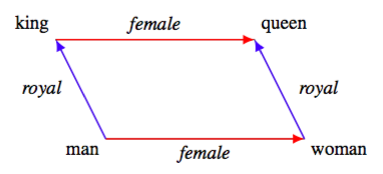
\includegraphics[width=0.5\linewidth]{sources/related_works/imgs/parallelograms_kawin.png}
    \caption{Illustration of the linear representation hypothesis as mentioned in \citet{mikolov-etal-2013-linguistic} (taken from \citet{ethayarajh-etal-2019-towards})}
    \label{fig:parallelo}
\end{figure}

A fundamental concept in neural model interpretability (and particularly for language models) is the linear representation hypothesis, i.e. the observation that \textit{high-level concepts are represented linearly as directions in [the] representation space} \citep{park2024the}.

This hypothesis was famously invoked in the Word2Vec article\footnote{The claim is usually attributed to Word2Vec but was initially made in an article from the same first author.} \citep{mikolov-etal-2013-linguistic}, where authors argued that arithmetic operations between the representations almost perfectly captured semantic relationships. For instance, they have been shown to capture analogies, as in the notorious example:
$$
x_{\text{queen}} \simeq x_{\text{king}} - x_{\text{man}} + x_{\text{woman}}
$$

This observation was explored and justified mathematically in the context of static word embeddings \citep{ethayarajh-etal-2019-towards, pmlr-v97-allen19a}. Recently, \citet{jiang2024on} showed that training a probabilistic model by optimizing cross-entropy via gradient descent theoretically pushes for a linear representation of underlying concepts, which generalizes the mathematical grounding of this hypothesis to representations of neural LMs. 

Most importantly, the linear representation hypothesis implies that self-supervised neural models can be \textit{probed} using linear methods in order to measure the extent to which a given concept is embedded in their representations. 

Typically, given $d$-dimensional frozen hidden representations modeled by a random variable $h$ and associated labels (respectively values) $y$ corresponding to a given concept, the \textit{linear probing} technique amounts to optimizing a linear (or affine) model $f_\Psi$ for a classification (respectively regression) loss $l$, i.e.:
$$
\Psi^* = \argmin_{\Psi} \mathbf{E}_{h, y}(l(f_\Psi(h), y))
$$

The resulting performance of the probe $f_\Psi$ indicates to what extent the representations encode the given concept. For instance, $h$ could encode sentence embeddings and $y$ could be a gender label for the subject in the sentence. Then, $l$ will be a classification loss, and $f_\Psi$ a trainable mapping from a representation $h_i$ to a gender prediction $\hat{y}_i$. In this example, he performance of the probe would indicate the amount of gender-related information that is encoded in the sentence representations.

\subsection{Embedded linguistic properties}
\begin{figure}[ht]
    \centering
    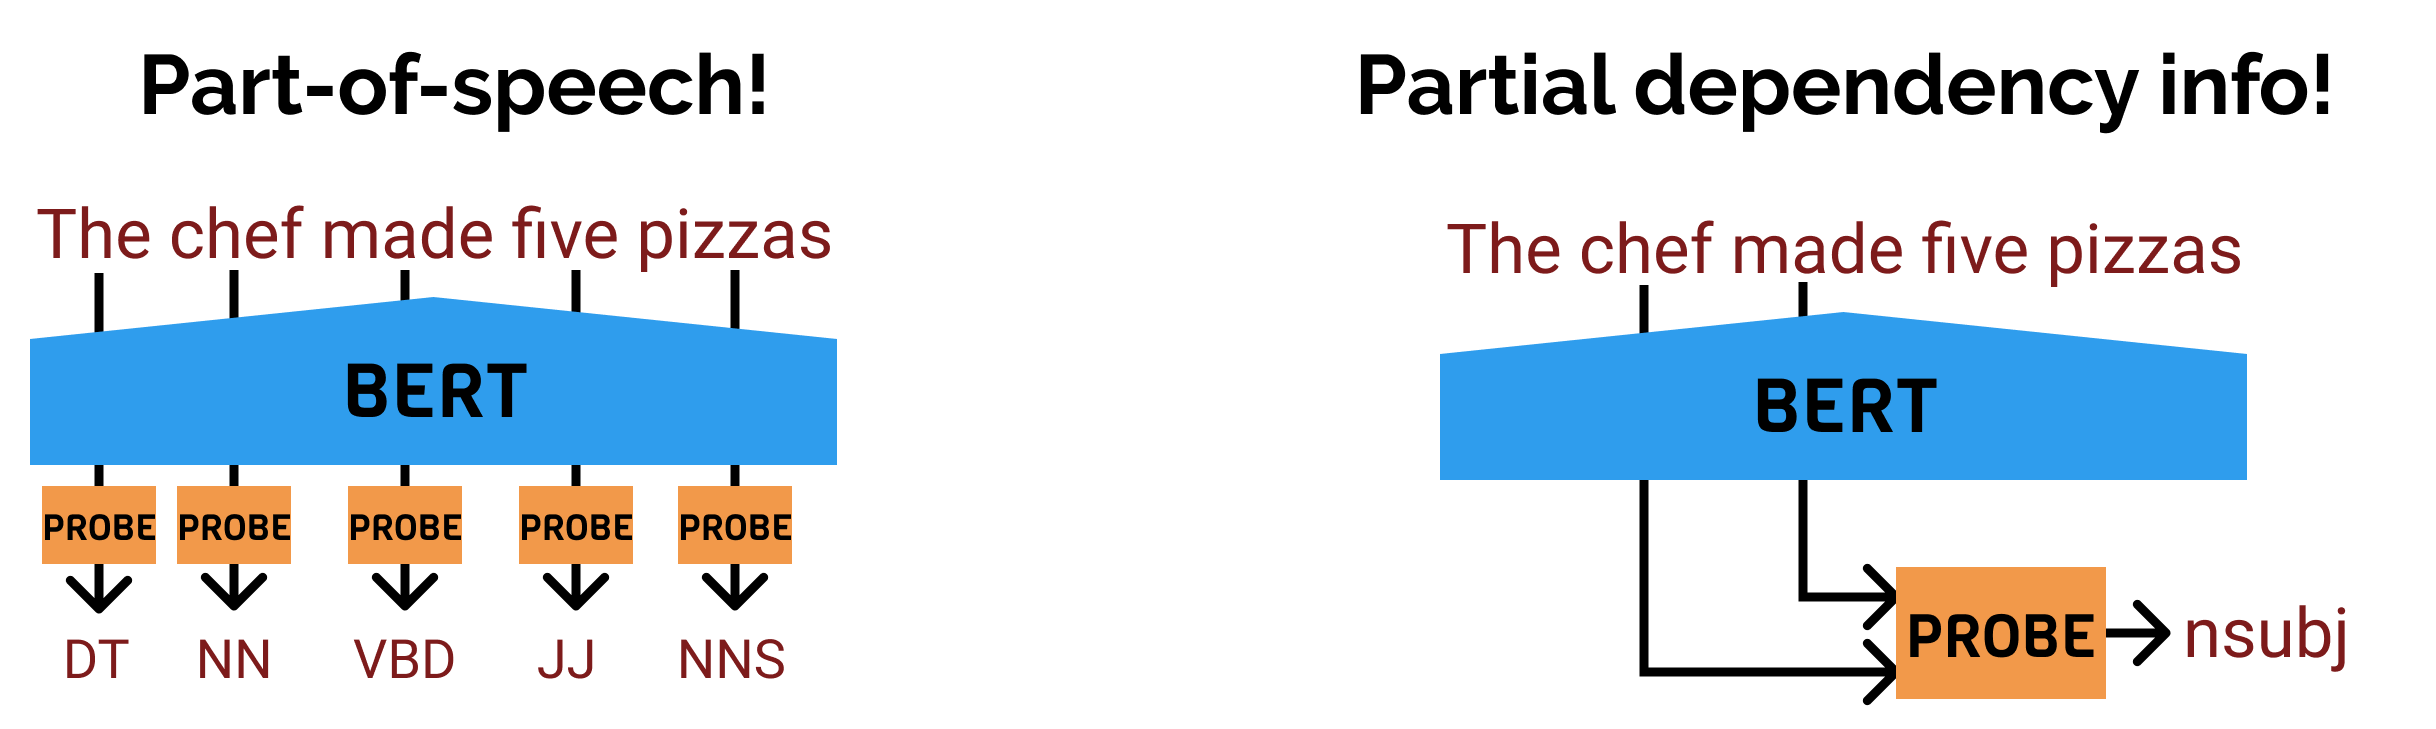
\includegraphics[width=0.7\linewidth]{sources/related_works/imgs/probing-diagram.png}
    \caption{A high-level summary of probing for language models (taken from \citet{Hewitt_2019})}
    \label{fig:probing}
\end{figure}



Early in the development of neural embedding methods, probing has been implemented to improve the understanding of how the representations capture information. \citet{kohn-2015-whats} successfully probe Word2Vec embeddings for basic word-level linguistic properties such as Part-of-Speech or gender. \citet{shi-etal-2016-string} show that RNN-based machine translation models partly learn the syntax of the source language using probing. \citet{adi2017finegrained} and \citet{conneau-etal-2018-cram} probe sentence representations from a linguistical point of view. They focus on relatively basic properties, such as the sentence length, or the belonging of a given token. \citet{liu-etal-2019-linguistic} extend this idea to token-level representations, and propose to use usual downstream tasks, such as POS tagging or Named Entity Recognition, as probing tasks. They train layer-wise probes and show that the necessary linguistic information is better contained in deeper layers.

These probing tasks have been used to better understand the layer-wise organization of neural LMs. \citet{peters-etal-2018-dissecting} show that the first layers focus on local syntax, while deeper layers focus on semantic content. \citet{tenney-etal-2019-bert} further decompose the roles of layers and find that the BERT model unsupervisedly mimics traditional NLP pipelines, i.e. it first latently parses the sentences before identifying coreferences and semantic relations. \citet{jawahar-etal-2019-bert} come to similar conclusions, but also notice that BERT is able to capture linguistic hierarchy and to mimic tree-like structures at representation level.



\subsection{Embedded world knowledge}


Several works have probed models in search for world knowledge, in order to quantify the ability of LMs to learn meaningful representations of physical objects beyond linguistic semantic.

\citet{gupta-etal-2015-distributional} show that static representations contain referential information about named entities. For instance, it is possible to roughly estimate population count, geolocation and other properties from city or country names using a basic probe.

Subsequently, different works have studied temporal knowledge \citep{thukral-etal-2021-probing, caselli-etal-2022-time}, auditive representations \citep{ngo2024languagemodelshearprobing} or factual knowledge \citep{youssef-etal-2023-give}, among others. In this work, we focus on geographical knowledge, and wonder whether geo-localisation information is embedded in the representations of geographical entities.

\citet{lotr} show that coordinates of places in the Middle-Earth can be predicted by just using the co-occurence matrix extracted from the Lord of the Rings novels. \citet{faisal-anastasopoulos-2022-geographic} build networks from geographical representations based on monolingual and multilingual models of different sizes. They show that all models embed more accurate geographical representations for countries of the Global North. This geographical discrepancy can be explained by biases that are inherent to the datasets used for pretraining \citet{faisal-etal-2022-dataset}.

Recently, \citet{gurnee2023language} probed large language models from the Llama-2 suite \citep{touvron2023llama} to extract coordinates of prompted locations from hidden representations across layers. They show that models ranging from 7B to 70B parameters are able to convincingly embed geographical coordinates on a world map when representing basic prompts. They prove that scaling up the model size systematically leads to better performance in coordinates prediction.

\citet{peters-etal-2019-knowledge} propose to use the probe loss as an auxiliary objective during training, explicitly encoding chosen properties in the representations. They argue that the resulting model is more performant on downstream tasks after fine-tuning.

A concurrent line-of-work rather focuses on the analysis of data-inherent socio-cultural biases in models at representation-level. Instead of probing encyclopedic world knowledge, these methods evaluate the extent to which language models are contaminated by the stereotypical views that belong in natural language, or by statistical imbalances that may implicitly reinforce these views in these models.

\citet{zhao-etal-2018-gender} study gender bias in co-reference resolution systems. Co-reference resolution is a linguistic task that consists in indentifying the object of a reference (a pronoun referring to a past name for instance) that could potentially seem ambiguous. Analyzing the errors made by a coreference resolution system can provide insights about its underlying representations of concepts. For instance, let us consider the sentence ``\textit{the physician hired the secretary because she was overwhelmed with clients}''. A model that wrongly predicts that \textit{she} refers to \textit{secretary}, but would predict the correct reference when replacing \textit{she} with \textit{he}, likely suffers from stereotypical gender biases. They propose to quantify gender bias more directly in static embeddings by measuring the cosine similarity between the gender token (e.g. \textit{female}) and attributes like profession tokens (e.g. \textit{colonel}) \citep{zhao-etal-2018-learning}.

\citet{zhao-etal-2018-learning} go further and introduce auxiliary objectives to the GloVe method that help minimize their bias metric, which implies minimizing the alignment between some attributes and gender in the token-level representation space. In a similar effort, \citet{ravfogel-etal-2020-null} post-edit statistical embeddings by iteratively projecting them on the orthogonal direction of a trained linear probe. Intuitively, training a new probe on these projected embeddings should be more difficult as a gender-sensitive direction has been suppressed from the latent space. \citet{iskander-etal-2023-shielded} extend this idea to more complex probes and introduce a gradient-based method of which \citet{ravfogel-etal-2020-null} is a particular case.





\section{Analysis of Self-Attention}

After the emergence of Transformer-based models, many interpretability works have focused on the multi-head self-attention layers. These layers differ from the other linear layers as they model the interactions between tokens.

\subsection{Properties of self-attention maps}

When attention was introduced as a way to improve machine translation neural systems \citep{bahdanau_nmt}, it was shown that cross-attention maps were implicitly modeling token-to-token cross-lingual mappings. 

The self-attention patterns of BERT have been analyzed in numerous works. \citet{clark-etal-2019-bert} describe head-specific patterns, such as attending to punctuation, special tokens used for self-supervision (e.g. \texttt{[SEP]} or \texttt{[CLS]}), and previous or next tokens. They also identify a pattern with the entropy of head-level attention maps, where lower layers contain high-entropy maps that roughly average the representations of all token positions. They proceed by identifying specific heads that specialize in extracting a specific type of linguistic phenomenon through attention maps. They use attention maps and GloVe embeddings as an input to a dependency parsing classifier, and obtain satisfying results, showing that attention maps latently perform operations that are related with parsing.

\citet{voita-etal-2019-analyzing} conduct a similar analysis and find that pruning non-specialized heads does not significatively affect performance in Transformer-based machine translation. \citet{vig-belinkov-2019-analyzing} concurrently identify head-specific patterns on GPT-2 \citep{gpt2}, and add that deeper layers tend to encode longer-term dependencies than first layers.

Overall, these works show that self-attention maps in language models tend to be sparse (or low-entropy), which can make them easily interpretable in some cases. Quantitavely, head-level probing tasks and downstream evaluation allows to measure and characterize their specialization from a linguistic point of view.

\subsection{The logit lens}

\begin{figure}[ht]
    \centering
    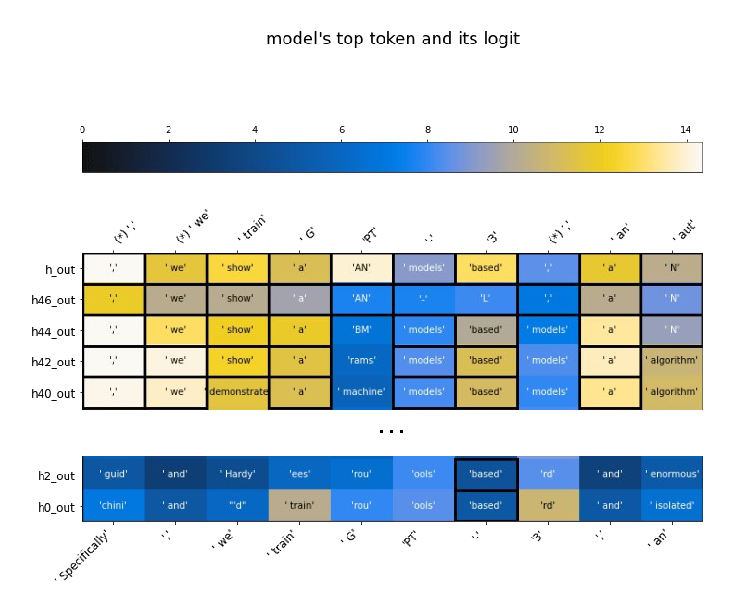
\includegraphics[width=0.7\linewidth]{sources/related_works/imgs/logit_lens.pdf}
    \caption{Layer-wise diagram obtained with the logit lens technique (taken from \citet{logit_lens})}
    \label{fig:probing}
\end{figure}

Although the methods mentioned above are efficient at measuring the quantitative linguistic performance of specific parts of Transformer models, they depend on a biased evaluation protocol, as the tasks and measurements are made with a specific angle of study. This remark led to the elaboration of techniques that automatically discover interpretable patterns.

\citet{logit_lens} introduce the concept of \textit{logit lens} \citep{logit_lens}, a projection technique that allows to extract token-related interpretations from intermediate representations in Transformer blocks. They observe that the residual connections of Transformer architectures create direct paths to the last hidden representation, which is then simply projected linearly on a $V$ dimensional logit space by the language modeling head. Hence, they hypothesize that the structures of the representations that go through these residual connections are suited for the language modeling head, implying that projecting them through this layer will produce meaningful outputs in the logit space. They mostly use this observation to analyze the stacked layers as improving predictors and to display their intermediate predictions.

\citet{elhage2021mathematical} develop a more elaborate framework around a similar idea, and identify \textit{circuits} in Transformer models, i.e. paths through the layers via a residual stream that processes specific features with each linear operation

\citet{prakash-lee-2023-layered} use the logit lens technique on large LMs to investigate the semantic changes that occur after bias mitigation techniques \citep{ravfogel-etal-2020-null}. \citet{dar-etal-2023-analyzing} design an equivalent framework to analyze model weights in the token space.

These initiatives tend to show that Transformer layers all contribute to the final prediction through a residual stream, where some heads sparsely process input representations in an interpretable way. Once more, these sparse implicit operations happen in linear subspaces that can be analyzed in token space via basic operations.

\subsection{QKV geometry}
To the best of our knowledge, few works have specifically studied the vector distributions of attention-level representations $Q^h$, $K^h$ and $V^h$.

Recently, \citet{devoto2024simpleeffectivel2normbased} observed that the $L_2$ norm of the $K^h$ representations could be used as a proxy for subsequent attention weights. They derive an efficient KV cache compression scheme from this observation, proving that $K^h$ representations with the highest $L_2$ norm can actually be discarded at inference time without significant performance loss.

\section{Representation degeneration}
\label{sec:rw_degeneration}

Representation Degeneration is a phenomenon in which pretrained models tend to adopt low-entropy singular value distributions \citep{jing2022understanding}. In other words, the singular value distributions of the representations of affected models are particularly imbalanced, which implies that they can be efficiently approximated in a lower-dimensional subspace.

In language modeling, representation degeneration has been studied from various points of view, and specificities related to the (Zipfian) distribution of textual data have been put forward to explain the forms of degeneration that were observed at various levels in models. Hence, we argue that representation degeneration can be included in the field of interpretability, as it depicts distortions that may be explained by general properties of natural language.

We summarize the works that cope with this question in the following sections.

\subsection{A general phenomenon}

\citet{9709917} identify dimensional collapse as a potential caveat of self-supervised models in general. They suggest that features tend to naturally collapse towards highly dependent patterns. To measure this phenomenon, they track several metrics for the generated representations. They estimate the rank of the space spanned by the representations by computing the singular values of a representation set, and show that this estimated rank tends to decrease in training. They also measure the average absolute correlation scores across features, and show that this correlation does not naturally decrease. 

A way to circumvent this phenomenon is to penalize feature similitude, which they implement through a covariance regularization term. \citet{pmlr-v139-tian21a} show that architectural tricks such as weight decay \citep{weight_decay} or exponential moving averaging \citep{morales-brotons2024exponential} can mitigate dimensional collapse.

Another natural approach towards mitigating dimensional collapse is contrastive learning, as it implicitly improves the uniformity of latent spaces \citep{pmlr-v119-wang20k}. Nevertheless, \citet{jing2022understanding} show that for a broad range of data augmentation techniques used when generating positive samples, contrastive methods lead to dimensional collapse. They design architectural tricks and improved data augmentation methods to alleviate this issue.

Most importantly, in agreement with \citet{pmlr-v119-wang20k}, these works notice that uniformity in latent spaces is correlated with performance, and that mitigating dimensional collapse leads to better models in general.

\subsection{Degeneration in NLP}
\label{ssec:degeneration}

\begin{figure}[ht]
    \centering
    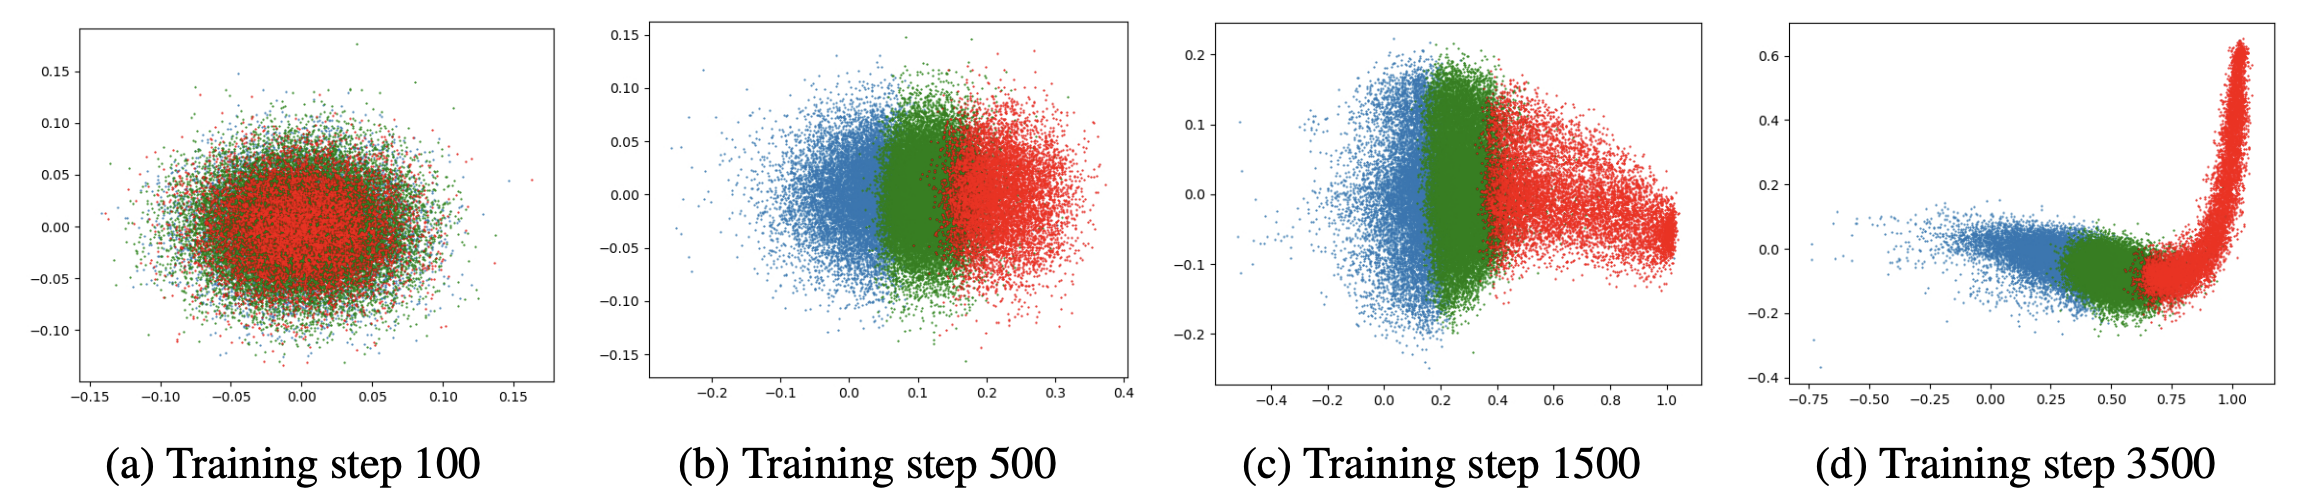
\includegraphics[width=0.9\linewidth]{sources/related_works/imgs/freq_degen.png}
    \caption{Visualization of the token embeddings of a language model during training, projected onto the first two components of their SVD. Red, green, and blue points represent rare, medium, and frequent groups respectively (taken from \citet{yu-etal-2022-rare}). These plots show the emergence of a degeneration phenomenon and its apparent correlation with token frequency.}
    \label{fig:repr_vs_freq}
\end{figure}

In NLP, \textit{degeneration} is a term that has been used in various works to convey different meanings. 

Firstly, it has been used to describe erratic behaviors of language models at inference time, with notable examples of repeated tokens or phrases, and of strong hallucinations. \citet{Holtzman2020The}, describe the \textit{neural text degeneration} phenomenon in depth. Through extensive analysis of GPT-2 generated sequences, they show that pre-existing decoding methods, such as beam search \citep{freitag-al-onaizan-2017-beam}, temperature sampling \citep{ACKLEY1985147}, or top-k sampling \citep{gpt2}, all lead to undesirable outputs. They argue that ``\textit{natural language does not maximize probability}'', and that decoding methods that aim at purely minimizing the perplexity of the model on the generated text are bound to lead to less human-like samples. They introduce nucleus sampling, a strategy that thresholds the token distribution based on its cumulated distribution function (CDF). \citet{Welleck2020Neural} suggest an alternative method that consists in continue the training of the model with an auxiliary \textit{unlikelihood} loss that explicitly penalizes repetition and induction-based hallucinations.

\citet{finlayson2024closing} investigate the implication of the softmax bottleneck (see \Cref{ssec:softmax_bottleneck}) in this kind of degeneration, and show that the low-dimensional linearity of the language modeling head may introduce artifacts in the next-token probability distributions. As a matter of fact, they argue that when the hidden dimension $d_m$ is smaller than the vocabulary size $V$, the logits vector lie in a space spanned by the language modeling head, which is a relatively low-dimensional manifold of $\mathbb{R}^V$. As a result, projecting these logits on $\Delta^V$ using the softmax function leads to spurious non-zero probabilities for tokens that would be null otherwise, as the low-dimensional manifold cannot be mapped to $\Delta^V$ in a surjective manner. This phenomenon explains the efficiency of truncation strategies such as nucleus sampling, as they will discard most of the spurious non-null probability tokens when the error caused by the softmax bottleneck is not too significant.

\citet{scaling_manifold} also link the performance of language models to the dimensionality of hidden representations and of the data distribution itself. They argue that the parameters of the scaling laws (see \Cref{ssec:scaling_law}) can be esimated through a study of the \textit{intrinsic dimension} or ID \citep{intrinsic_d} of the data manifold. \citet{intrinsic_d} use \textit{persistence homology dimension} \citep{phdim}, a fractal dimension estimation metric based on minimal spanning trees, to measure the ID of embedding distribution of artificially generated texts and human text. They find that artifical samples tend to have a lower intrinsic dimensionality than human samples. \citet{scaling_manifold} use a similar metric to estimate the data dimensionality, and to verify their approximation of the scaling laws based on this measure.


The notion of \textit{degeneration} has also been used to extend the exploration of representational degeneration to the specific case of natural language modeling. A seminal work in that field is \textit{Representation Degeneration Problem in Training Natural Language Generation Models} \citep{gao2018representation}. In this paper, the authors underline a connection between the distortion that can be observed in both static and contextual embeddings spaces, and the unbalanced Zipf law that appears in natural language.

They elaborate their claim around the example of an unused token, that is a token that belongs in the vocabulary $\mathcal{V}$ of the language model, but that does not appear in the training sequences. This can happen if the tokenizer and the model are trained on different datasets. Let's consider the case where there is only one such token $w_u$, and all the model $\theta$ parameters are fixed except for the parameters of the language modeling head $W_o$, of rows $(o_i)_{i\in[1, V]} \in \mathbb{R}^{V \times d_m}$. The authors focus on the parameters $o_u$, which are updated during training to optimize the cross-entropy loss, in a \textit{consistent} way where the output logit for $w_u$ must be as low as possible as $w_u$ never appears. More formally, if a set of $\Upsilon$ contextual embeddings from the frozen model are noted $(h_i)_{i \in [1, \Upsilon]}$, optimizing cross-entropy with respect to $o_u$ amounts to the following problem:
$$
\argmax_{o_u} \frac{1}{\Upsilon} \sum_{i=1}^{\Upsilon}\left(\log \frac{\exp \langle h_i, o_{w_i} \rangle}{\sum_{j\in[1, V] \setminus u} \exp \langle h_i, o_{j} \rangle  + \exp \langle h_i, o_u \rangle}\right)
$$
which can be reduced by introducing a constant $C_i$, to :
\begin{equation}
    \label{eq:min_unused}
    \argmin_{o_u} \frac{1}{\Upsilon} \sum_{i=1}^{\Upsilon}\log \left(C_i  + \exp \langle h_i, o_u \rangle\right)
\end{equation}

\Cref{eq:min_unused} shows that the parameters corresponding to $w_u$ in the language modeling head are trained to minimize an average metric on the whole dataset, that naturally pushes the scalar products $\langle h_i, o_u \rangle$ towards negative values. The authors show that this optimization problem tends to lead to a degenerate solution where $o_u$ is pushed away from the convex hull of the representations~$\mathbf{h}$.

They extend this observation to rare tokens through more complex analysis, and deduce that training a model using cross-entropy on data that has an underlying Zipfian distribution naturally leads to a distortion of the output latent space. Frequency-based degeneration was also observed in \citet{zhou2021frequencybaseddistortionscontextualizedword}, who show that the representational geometry of tokens is highly dependent on their frequency, and that rare tokens are less distinguishable in latent spaces. They argue that this difference can explain biases in downstream performance, using the example of geographical knowledge discrepancy between high-frequency and low-frequency location names.

To overcome this limitation, \citet{yu-etal-2022-rare} train a language model using adaptive gradient gating, which regularizes the gradients related to low-frequency tokens. \citet{meister-etal-2023-natural} propose a simpler approach where a bias is added to the output of the language modeling head. This bias is manually set to $b_i = \log(f_{w_i})$, where $f_{w_i}$ is the unigram frequency of token $w_i$, which allows the model to only model a residual contribution to the contextual probability, making it less sensitive to token frequency.

\subsection{Anisotropy \& Outlier Dimensions}


\begin{figure}[ht]
    \centering
    \begin{subfigure}[b]{0.3\textwidth}
        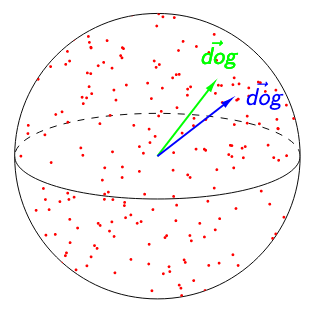
\includegraphics[width=\textwidth]{sources/related_works/imgs/anisotropy_kawin.png}
        \caption{Isotropic distribution}
        \label{fig:iso}
    \end{subfigure}
    \begin{subfigure}[b]{0.3\textwidth}
        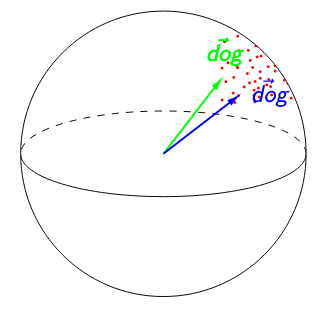
\includegraphics[width=\textwidth]{sources/related_works/imgs/anisotropy_kawin_2.png}
        \caption{Anisotropic distribution}
        \label{fig:aniso}
    \end{subfigure}
    \caption{Schema of anisotropy in a token embedding space. (taken from \citet{ethayarajh-2019-contextual})}
    \label{fig:anisotropy}
\end{figure}


A specific framing of representation degeneration in language modeling has taken the form of \textit{anisotropy}, that is of non-uniformity of the distribution of angular components in language model representations. 

To the best of our knowledge, \citet{ethayarajh-2019-contextual} is the first to describe this phenomenon for contextual representations in natural language. He defines anisotropy as the average cosine similarity between two randomly sampled representations at a given layer. Formally, if $\Upsilon$ outputs representations $\mathbf{h}^i$ are uniformly sampled from the $i$-th layer of a neural network, then the anisotropy level of that layer can be measured as:
\begin{equation}
    \label{eq:anisotropy_cos_def}
    \mathcal{A}_{cos}(\phi_\theta, i) = \frac{1}{\Upsilon^2 - \Upsilon} \sum_{n \neq m} \frac{\langle h^i_n, h^i_m \rangle}{||h^i_n||_2 \cdot||h^i_m||_2 }
\end{equation}

$\mathcal{A}_{cos}(\phi_\theta, i)$ takes a value in $[-1, 1]$, and the distribution of $\mathbf{h}^i$ can be described as anisotropic when $|\mathcal{A}_{cos}|$ takes higher values.

They measure anisotropy on hidden representations obtained across different sentences using this in ELMo \citep{peters-etal-2018-deep}, BERT \citep{devlin-etal-2019-bert} and GPT \citep{Radford2018ImprovingLU}. They find that hidden representations of these models tend to be anisotropic, especially on the deeper layers, and notice that the anisotropy level of GPT takes extreme values (up to $0.97$). In simpler terms, when sampling two output token representations of GPT at random (across documents or not), the cosine similarity between these will be $0.97$ in average. This is unexpected, as a uniform distribution would likely yield orthogonal vectors, especially in high-dimension settings.

\citet{mu2018allbutthetop} explore anisotropy from the perspective of singular value decomposition. They measure an average similarity between each singular vector $u^i \in U^i$ and each hidden representation $h^i$, and by comparing the maximum average similarity (the singular component that is most similar to hidden representations) and the minimum average similarity (the singular component that is least similar to hidden representations). In an isotropic distribution, these similarity levels should be closer as each singular component should almost equally explain all hidden representations. The precise measure is done as such:
$$
\mathcal{A}_{SV}(\phi_\theta, i) = \frac{\min_{u \in U} F(u)}{\max_{u \in U} F(u)}
$$
where $F(u) = \frac{1}{\Upsilon} \sum_{t=1}^{\Upsilon} \exp (\langle u^i, h^i_t\rangle)$.

Here, $\mathcal{A}_{SV}(\phi_\theta, i) \in [0, 1]$ and the distribution is characterized as anisotropic when it is significantly smaller than $1$. They use this measure to show that static embeddings to be anisotropic, and they propose a basic truncation of top singular components to improve their anisotropy. They show that the resulting isotropic static embeddings lead to better performance on downstream tasks.

\citet{Wang2020Improving} take advantage of this spectral viewpoint and use spectrum control to mitigate anisotropy during training. They add a penalization term in the training objective that sets a target for the singular value distribution of the representations. They show that this regularization leads to better performance for language models in monolingual and mutlilingual setups, including for downstream performance.

\citet{rajaee-pilehvar-2021-cluster} use this metric on pretrained language models and come to similar conclusions to \citet{ethayarajh-2019-contextual}. They observe that the spaces spanned by $\mathbf{h}^i$ vectors are split into clusters which may cause anisotropy. They cluster the representations using unsupervised techniques, and compute the clusters barycenters before substracting them from their representations. They show that this post-processing step improves both the STS performance and the results on the NLI benchmarks, while successfully mitigating anisotropy. \citet{rajaee-pilehvar-2022-isotropy} extend the anisotropy diagnosis to the multilingual version of BERT. \citet{haemmerl-etal-2023-exploring} later propose several post-processing techniques to mitigate anisotropy, and show that they improve the performance of sentence embeddings.

\citet{bis-etal-2021-much} prove the existence of a connection between this anisotropy phenomenon and a degeneration similar to the one described in \citet{gao2018representation} (see \Cref{ssec:degeneration}). They show that training language models through cross-entropy optimization leads to a progressive drift of the embeddings towards a common direction, and that such a drift can be measured as an increase in anisotropy levels as a non-centered representation distribution is naturally contained in a narrower region of the space. They remove this common component by substracting the average representation, and show that this simple operation substantially reduces the anisotropy of the distributions according to $\mathcal{A}_{cos}$. Crucially, this connection allows them to formally bridge frequency-related distortions of the embedding space and anisotropy.

Several approaches have taken an opposite stance and have suggested that anisotropy was unharfmul and could even lead to better performance. \citet{ait-saada-nadif-2023-anisotropy} show that anisotropy does not affect clustering performance in sentence representations. \citet{rudman2024stable} propose to add an \textit{isotropy} penalization in the training objective of language models when fine-tuning on downstream tasks, and show slight performance improvements. Finally, \citet{machina-mercer-2024-anisotropy} show that anisotropy does not automatically appear in the output layers of larger language models.


A problem that is closely related to anisotropy is the existence of outlier dimensions in the representations of language models, which are also related with token frequency \citep{puccetti-etal-2022-outlier}. However, outlier dimensions are a form of anisotropy themselves, and most of the mitigation techniques that have been proposed in this subfield are related with quantization issues \citep{ahmadian2023intriguing,nrusimha2024mitigatingimpactoutlierchannels}. Hence, we choose not to include this literature in detail in this section.


\vspace{2em}

The aforementioned works cover diverse topics and aim for different objectives. Nevertheless, they tend to focus on the geometrical interpretability of language models in the representational space. These works show that viewing the activations of these models as vectors that should lie in meaningful spaces can bring performance improvements when leveraged properly. Understanding the geometry of these spaces with respect to data-related properties allows to better understand the behavior of a model, but also to point out limitations that the language modeling paradigm brings, when these spaces are not uniform or when they are too constrained to lead to optimal predictions.
